\documentclass[12pt,oneside]{fithesis2}
\newenvironment{changemargin}[2]{%
\begin{list}{}{%
\setlength{\topsep}{0pt}%
\setlength{\leftmargin}{#1}%
\setlength{\rightmargin}{#2}%
\setlength{\listparindent}{\parindent}%
\setlength{\itemindent}{\parindent}%
\setlength{\parsep}{\parskip}%
}%
\item[]}{\end{list}}
\usepackage[english]{babel}
\usepackage[utf8]{inputenc}
\usepackage[T1]{fontenc}
\usepackage{fixltx2e}
\usepackage[plainpages=false,pdfpagelabels,unicode]{hyperref}
\usepackage{indentfirst}
\usepackage{setspace}
\usepackage{listings}
\usepackage{lscape}
\usepackage{enumitem}
\usepackage{tabularx}
\usepackage{graphics}
\usepackage{epstopdf}
\usepackage{float}
\usepackage{mathtools}
\thesistitle{Real-time collaboration in Komodo} 
\thesislogo{fi-logo.mf}
\thesissubtitle{Master's thesis}
\thesisstudent{Bc. Matúš Makový} 
\thesiswoman{false} 
\thesislang{en} 
\thesisfaculty{fi}
\thesisyear{Spring 2015}
\thesisadvisor{RNDr. Filip Nguyen} 
\setstretch{1.2}
\begin{document}
\FrontMatter
\ThesisTitlePage
\begin{ThesisDeclaration}
\DeclarationText
\AdvisorName
\end{ThesisDeclaration}
\begin{ThesisThanks}
%Thank you
\end{ThesisThanks}
\begin{ThesisAbstract}
%Abstract
\end{ThesisAbstract}
\begin{ThesisKeyWords}
%Keywords
\end{ThesisKeyWords}
\tableofcontents 
\MainMatter
\chapter{Introduction} 
Many software solutions enable people to create new things in a better and faster way. In most cases the resulting product should be so complex that one person is not enuogh for the successful and fast creation. Creators try to collaborate to achive a common goal. Among other opportunities and possibilities are collaboration and sharing the greatest benefits of the Internet. \par
We can identify two types of collaboration over the Internet, non real-time collaboration and real-time collaboration. 
\par At the beginning, as the Internet didn't have such capacity, people tried to use it just for sharing their drafts of work and sending them to each other, this type of collaboration is called non real-time. In non real-time collaboration users work on separate copies of a project and then need to merge their changes into one final project. In other words, they had to find differences between their drafts and reflect them to each other's version. It doesn't offer such flexibility as real-time collaboraion and also it had many limitations, for example two people could not edit the same file in a project without having to resolve confilicts manualy when they tried to merge their work with collaborator's version\par
Example of non real-time collaboration could be Revision control (Git, SVN).
With the development of the Internet came a reasonable solution called real-time collaboration. Using this principle, author can see what his collaborator is doing in real-time and the manual synchronization or manual confilict resolution is not necessary. Information technologies take care of this synchronization and conflict resolution for the users.
\par In the theoretical part of this thesis, we deal with principles of real-time collaboration and describe three of the techniques used to implement real-time collaboration in software over the Internet. In the following chapter, we set a comparison cirteria and try to compare these techniques in general. 
\par The practical part of this thesis presents a brief description of Red Hat JBoss Data Virtualization and Teiid Designer and also presnets Komodo software as a new version of Teiid Designer. Komodo should use real-time collaboration in its upcomming release. We present the requirements of this software on the technique and recommend best one for this authoring software and find a suitable implementation in Java programming language.

\chapter{Real-time collaboration}
This chapter covers the basic overview of collaboration in general, description of real-time collaboration and description of difficulties with its implementation over the Internet. Last sections of this chapter describe three techniques used for implementation over the Internet and its properties. Techniques described in this chapter are: Operational Transformation, Differential Synchronization and Commutative replicated data types.
\section{Basic overview}
Collaboration, as defined by English dictionary, is an act of working with another or others on a joint project. Authoring Systems in IT that support collaboration are called Groupware. \par "Groupware systems are computer-based systems that support \\two or more users engaged in a common task, and that provide an interface to a shared environment. These systems frequently require fine-granularity sharing of data and fast response times." \cite{Ellis} \par There are many techniques used in groupware systems that are not suitable for real-time collaboration, for example, Locking or Single Active Participant technique. Fundamental principle of Locking and Single Active Participant is to lock data when it is being modified by someone. This principle is adopted for example by Microsoft, when users try to edit shared document. \par When using real-time collaboration, authorig software creates an illusion that users are working on one common copy of a document online. There is no requirement to commit changes to some kind of shared repository and no need for a user to resolve conflicts. Changes should be reflected and saved immediately. Examples of real-time collaborative editors that we recognize today are Google Docs,\\ Etherpad and already terminated Google Wave. \par Software engineer has different options for implementetation of real-time collaboration in software solution. \par Requirements for a good technique are: 
\begin{itemize}
\item speed
\item latency tolerantion
\item low data transfer
\item consistency maintanance
\item good conflict resolution
\end{itemize}
\par The speed requirement means that changes made on one side of the collaboration process need to be reflected to the other sides as soon as possible and vice versa. Changes should be sent to other collaborators as soon as they are done. If a collaboration technique is fast enough it is much easier to satisfy other requirements on this technique. Fast enough technique is able to maintain good consistency. "The system’s response time is the time necessary for the actions of one user to be reflected by their own interface; the notification time is the time necessary for one user’s actions to be propagated to the remaining users’ interfaces." \cite{Ellis} Response time and notification time should be as short as possible.  \par One of the problems of real-time collabarative editing could be the latency of network. Implemented technique should be able to tolerate the latency of internet connections, because collaborators could be in very distinct parts of the world. It should be able to reconstruct the right order of operations because data sent over the Internet don't necessary come in right order and the order of the operations is very important to maintain consistency.\par Low data transfer requirement is also very important. Different sides of the collaboration should send as few data as possible. Transfered data should only describe change that has been done on one side of collaboration, it is not necessary to transfer the whole project. The less data is needed to transfer the faster the whole protocol can be.  \par Consistency maintanance is necesssary for the success, it has to be ensured, that users on both sides are looking and the same version of a document regardless of number and coplexity of operations done on both sides of the collaboration. Lack of consistency could cause other problems and chaos in the document versions. According to \cite{Vidot} there are three problems encountered when trying to achive consistency maintenance and they correspond to the properties of CCI consistency model proposed in \cite{Sun}
\begin{enumerate}
\item \textbf{Casuality Preservation} - operation \(O_{1}\) causually precedes operation \(O_{2}\) if \(O_{1}\) occured localy before \(O_{2}\). The problem is to execute operations in right order on all sites.
\item \textbf{User Intension Preservation} - technique must preserve user's intension in the context of state, in which the operation was executed. This problem is in strog relation with confilict resolution requirement and occures when it is not posible to determine if \(O_{x}\) casually precedes \(O_{y}\) or \(O_{y}\) casually precedes \(O_{x}\).
\item \textbf{Convergence} - when same operations have been applied on every site, the documents are identical.
\end{enumerate}
\par Because the real-time collaboration should be asychnronious there rises a problem of concurency. This means, that changes can happen at the same time and in the same sections of project. Good conflict resolution requirement is present because of concurency. Implementation techniques have to be able to identify and resolve a conflict when users are editing the same part of the project. \par The concurrency control algorithms are separeted in two classes: pessimistic and optimistic. \par "Pessimistic algorithms require communication with other sites or with a central coordinator before making a change to data." \cite{Jupiter} One example of pessimistic algorithm can be already mentioned Locking or Single Active Participant technique. \par "Optimistic concurrency control, on the other hand, requires no communication before applying changes locally. The party making a change applies it immediately, then informs the other parties of the action. If more than one participant makes a change at the same time, a conflict resolution algorithm creates compensating changes to move everyone to the same final state." \cite{Jupiter} \par This implies that optimistic algorithms are better solution for Internet, because the latency can not be guaranteed. 
\section{Operational Transformation}
\par Operational transformation (OT) is optimistic concurrency control algorithm used for real-time collaborative editing over the Internet. 
\par It was first introduced in paper Concurency Control in Groupware Systems \cite{Ellis} in 1989, together with The Distrubeted Optional Transformation (dOPT) Algorithm. "The algorithm has a number of properties which make it suitable for groupware. First, operations are performed immediately on their originating site, thus responsiveness is good. Secondly, locks are not necessary so all data remains accessible to group members. Finally, the algorithm is fully distributed, and resilient to site failure..."\cite{Ellis} \par This first algorithm was able to process only plain text. Later some problems with correctnes were discovered and resolved in following works. Over the years many other algorithms implementing OT have been published. Algorithms used today are able to process also XML and other formats. \par OT was used also in Jupiter Collaboration System in 1995 \cite{Jupiter}. Jupiter's two-way algorithm is derived from the dOPT algorithm used by Grove in \cite{Ellis}. This algorithm is one of the imporovments of dOPT. \par Today is Google one of the most common implementators of this protocol. The main application was in Google Wave project, which is now terminated , although Operational Transformation found application also in Google Docs project. According to \cite{Spiewak} Google is one of the bigest inovators of this approach an it's biggest contribution is the idea of operation compositon, which is described later in this section. \par The approches differ also in the architecture, dOPT doesn't involve server in its design, but the recent algorithms use a central server that maintains its version of the document, coordinates the communication and broadcasts operations.
\par This section will explain basic principles of Operational transformation using Google version of the control algorithm, introduce some improvements added by Google and then point out the differences between the presented version and other versions like dOTP, Jupiter and TIPS. 
\par The basic idea is that data are replicated on every machine and the only information that is sent over the Internet are the operations. Data replication ensures good responsivnes in high latency enviroments. Wave's addition to OT are also annotations. "An annotation is some meta-data associated with an item range, i.e., a start position and an end position. This is particularly useful for describing text formatting and spelling suggestions, as it does not unecessarily complicate the underlying structured document format." \cite{Google} \par The main building block of this approach, as the name suggests, is an operation. Here are operations defined for use in Google Wave \cite{Google}:
\begin{itemize}
\item retain() - move cursor
\item insertCharacters() - inserts texts
\item insertElementStart() - inserts starting tag
\item insertElementEnd() - inserts end tag
\item deleteCharacters() - deletes text
\item deleteElementStart() - deletes starting tag
\item deleteElementEnd() - deletes ending tag
\item replaceAttributes() - replaces attributes in tag
\item updateAttributes() - updates attributes in tah
\item annotationBoundary() - describes changes in annotations
\end{itemize}
\par The operation is executed locally and then sent over the network to the server or to other peers, to execute the operation on their version of the document. Every object that can be changed in the document has its index for identification. Google Wave uses XML as format for storing information so as an object is considered a character in text and also a starting and terminating tag in XML structure (characters of tags are not considered elements). 
\par The second major part of this technique is a transformation function, that transforms operations. Operations which are sent over the network and recieved by server can not be executed directly on the server's version of the document, because the index of the desired element could be different in the local copy and in the server copy of the document and this can cause inconsistency and violation of User Intension Preservation. 
\par See Figure~\ref{fig:ot} with example for better explanation. For the purpose of this example, we will assume that we have one client that sends operations done on his local copy and a server that recieves operations from all peers and maintains server version of the document. 
\begin{figure}[H]
\caption{Example Operational Transformation}
\label{fig:ot}
\centering
\vspace{5mm}
\includegraphics{op1}
\end{figure}
Both of them start with text 'TAX' in their document. Pointer starts at index 0 and operation retain() shifts the pointer by number of indexes given as parameter. Client wants to add character 'E' so he executes operations:
\vspace{3mm}
\begin{verbatim}
retain(3);
insertCharacters('E');
\end{verbatim} 
\vspace{3mm}
In the meantime server recieved operation from other peer, that has inserted character 'S', so server executes operations:
\vspace{3mm} 
\begin{verbatim}
retain(3);
insertCharacters('S');
\end{verbatim}
\vspace{3mm}
Server and client exchange the operations. Different order and difference in indexes on both sides of the collaboration result in incosistent document state. String in first document is 'TAXSE' and string in second document is 'TAXES'.  In order to preserve user's intension and to reach correct result we have to transform this operations. The correct result after inserting letters 'E' and 'S' should be 'TAXES'. Server has correct version of the document, but client doesn't so we have to transform the operation sent by server to look like this:
\vspace{3mm}
\begin{verbatim}
retain(4);
insertCharacters('S');
\end{verbatim}
\vspace{3mm}
This transformation was helpful, but it is not enough. Now the client operation retains 3 characters, inserts new character and leaves cursor in front of last letter and the server operation retains 4 characters inserts character and leaves cursor behind the whole word. Client and server should end up in the same state. So it is necessary to transform also the client operation: 
\vspace{3mm}
\begin{verbatim}
retain(3);
insertCharacters('E');
retain(1);
\end{verbatim}
\vspace{3mm}
After this change the result of applying operations on both sides will be correct.\par More gernerally, if we have two operations \(O_{1}\) and  \(O_{2}\) we need a transformation function \textit{trasform}, such that: 
\begin{center}
\(transform(O_{1},O_{2}) = (O'_{1},O'_{2}) \quad where \quad O'_{2} \circ O_{1} \equiv O'_{1} \circ O_{2} \) 
\end{center}
In other words, the function takes two operations and transforms them against each other and the output of the function are two transformed operations, such that, if we have same strings on both sides a we apply \( O_{1} \) and \(O'_{2}\) on one side, and \( O_{2} \) and  \( O'_{1} \) on the other side, the resulting string is the same. 
\par "If an OT system is to support particular functionality, then it must be able to support certain transformation properties. For group editing and consistency maintenance, the system must support a transformation function known as Inclusion Transformation (IT). For group undo, where the effect of a previously executed operation is un-done at all sites, and all operations executed after it are all re-transformed, the system must support another transformation function known as Exclusion Transformation(ET). Inclusion Transformation transforms operation \( O_{A} \) against another operation \( O_{B} \) in such a way that the impact of \( O_{B} \) is effectively included. Exclusion Transformation transforms operation \( O_{A} \) gainst another operation \( O_{B} \) in such a way that the impact of \( O_{B} \) s effectively excluded." \cite{Leung} Problem described in the example could be also visualized as a "diamond problem". See Figure~\ref{fig:diamond1}
\begin{figure}[H]
\caption{Diamond problem - 1}
\label{fig:diamond1}
\centering
\vspace{5mm}
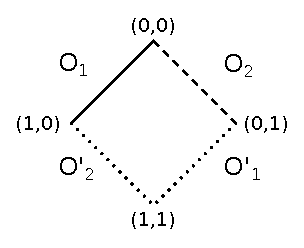
\includegraphics{diamond1}
\end{figure}
Operations done by peer take the document to the left side and operations done on server take the document to the right side. Each node in the diamond diagram represents the number of operations done by client and server in particular state. 
\par As for the example, the correct scenario would be that peer and server exchange their operations, each one computes its transformation and applies the transformated operation on their versions of documents.
\par The problem presented by this example is acctually the only one that is Operational Transformation capable of solving. Complicated situation occurs when sides of the collaboration diverge by more then one step. 
\begin{figure}[H]
\caption{Diamond problem - 2}
\label{fig:diamond2}
\centering
\vspace{5mm}
\includegraphics{diamond2}
\end{figure}
This example is used in \cite{Spiewak} On the server side, tranformation for operations \(a,c\) has to be computed, and server applies operation \(a'\) on its version of the document. The remaining operation \(c'\) has to be preserved for the next transformation. In the next step server must use \(b\) and \(c'\) as an input and computes \(b'\) that can be applied on its version of the document. Server's document is in the desired state. 
\par On the client side, \(c\) has to be transformed against two operations to get to desired state. For two operations it is not a big problem, but as the number of operations could very quickly increase, because Operational Transformation is an optimistic technique, so it could potecially take long time to process. One of the advantages of Google Wave Operational Transformation is that it is able to compose the operations if they are compatible. This Composer is able to validate operations to make sure that they are compatible and compose them. One of the criteria for comatibility is that operations must span the same number of indexes.  If operations \(a\) and \(b\) are composed into operation \(d\), tranformation function can take operations \(d,c\) and produce operation \(c''\) that can be applied to peer's document and the document is in desired state. 
\par This example is still simple. It does not point out some necessary parts of Operational transformation. The importance of preservation of operation \(c'\) was obvious from the diagram, but without the diagram it is hard to determine what operation should server or client preserve. In order to make it easier, metadata about the partent state of the operation is added. Every operation has an identificator of state in which it was executed. Google Wave uses a scalar version number, but \cite{Spiewak} suggests to use a hash of the documents contents. 
\par Having information about parent state, the server is able to determine that parent state of operation \(b\) is not in server history and it has to derive a new operation, that would take the document to state after application of operations \(a\) and \(c\). According to \cite{Spiewak} this operation is \(c'\). This deriving of operation \(c'\) is called bridgeing.
\par With this new feature comes a new problem. In order to derive the operation \(c'\) server has to preserve also operation \(a\). This could be a scalability problem in an enviroment with many clients editing the same document, since server has potecially preserve this data for every client. This is resolved by trasnfering all the resposibility to client and buffering the operations on client side. Client can send only operations that come from state in server's history and also he can send only one operation to the server and he has to wait for the acknowledgment of the operation. All following operations are preserved in buffer on client side. One of the advantages of buffering operations is that if this operations are compatible, they can be composed using the Composer. When the server ackwnoledges first operation, client can send next operation. This way client can predict servers path and send only operations that are on the servers path. Also it is much more complicated for the server to track every client, but it generall is much easier for client to track only one server. This way the server solves only one step diamond problem presented in the first example.
\par Daniel Spiewak in article Understanding and Applying Operational Transformation \cite{Spiewak} describes some other improvments of Operational Transformation by Google Wave. For example, when client recieves operation from server and has some operations in buffer, he can transform the whole buffer against this operation in order to accelerate the process on his site and also to ensure that operations in buffer have a parent state in servers history.
\par The main difference between Google control algorithm and the first dOPT algorithm is that dOPT doesn't use transformation function, it uses transformation matrix. If we have set of operations of cardinality m the matrix should be of size m x m. The entries of the matrix correspond to all possible pairs of operations and contain functions which transform operations to other operations. \par Another important part of the algorithm is the state vector. "Time\-stamps for each client are handled by a vector timestamp, where a state vector \(s_i\) for a client \(C_i \) will have at position \(j\), the number of operations known to have been executed by client \(C_j\)." \cite{Leung} \par According to this vector it is decided whether the recieved operation is executed or put in the request queue.
\par The difference between Google algorithm and Jupiter is not so significant. Actually, Jupiter also uses tranformation fucntion, it is called xform, although it is very similar to dOPT transformation matrix. Only differences is that Jupiter doesn't use the operation composition. According to \cite{Jupiter} this algorithm assumes use of transport layer that delivers data in right order, such as TCP.
\par The last major algorithm implementing this technique is TIPS, which is modern and based on the admissibility-based trasnformation (ABT) framework. It is created on top of HTTP protocol. Main difference is that clients can join and leave session at any time and the algorithm is more reliable when network failures can be expected. 
\section{Differential Synchronization}
\par Differential synchronization is the second technique used for real-time collaboration. It was fully described in 2009 by Neil Fraser in paper Differential Synchronization \cite{Fraser}. This section will describe and explain this technique, point out its advatages and disadvatages. As the main source of this information will be used paper mentioned above, because it is also the only article that fully describes this principle.
\par DS also replicates data on all sites of collaboration and identical code runs on both server and client, so it is symmetrical. The main building block is the presence of diff \& patch algorithms. Diff algorithm is able to compute a difference between to documents and save it in apropriate format for the patch algorithm, wich is able to apply these changes on the other copy. The patch algorithm must be fuzzy, this means that the changes may be applied even if the document has changed in the meentime, because Differential Sychronization is an optimistic technique. The final version presented by Neil Fraser is suitable for unreliable networks and networks with high-latency. This property will be described later in this section.
\par "The key feature of DS is that it is simple and well suited for use in both novel and existing state-based applications without requireing application redesign." \cite{Fraser} Differential Synchronization is able to process variety of formats, not only plain text. As long as there is a diff and patch algorithm available for the desired format, DS is able to use it. It is implemented and used in MobWrite. 
\par Basic priciple of this tehcnique can be described using data flow diagram in Figure~\ref{fig:ds1} originaly presented in \cite{Fraser}.  
\par In the begining Client text, Server text and Common Shadow are the same. Client text and Server text represent two sites of the collaboration. The goal is to keep them updated. Client and Server are allowed to make changes in their documents at any time. 
\begin{figure}[H]
\caption{Differential synchronization - Basic Architecture \cite{Fraser}}
\label{fig:ds1}
\centering
\vspace{5mm}
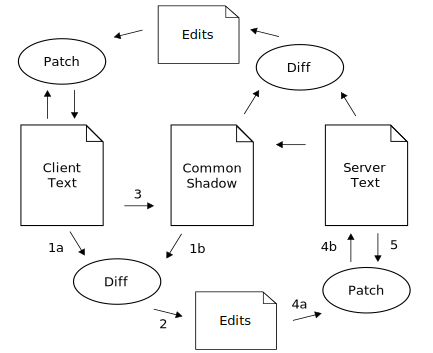
\includegraphics[scale=0.55]{diff1}
\end{figure}
After specified time interval (timeout) a snapshot of Client text is taken and using a diff algorithm the difference between client snapshot and common shadow is acquired. Common shadow represets the last common document state before any edits have been made. The output of these algorithms are changes that have been done by client. The client snapshot is copied over to the Common Shadow and the changes are patched on the Server text. Now the process repeats symmetrically using the server text in order to apply changes made by server or other clients on the client text. This time the Common shadow is the same as client snapshot, so diff algorithm returns changes made by server. The technique is very simple, it is obvious that the main parts of this technique are the diff a patch algorithms.
\par This example is suitable for explanation of the theory behind this technique, but not for use in practice. The problem is that the shadow is common and there is no method to implement this in real life. Client and server must have separate copies of "common" shadow. These copies are called Client Shadow and Server Shadow.
\par We have to make sure that Client Shadow and Server shadow are the same after every synchronization. The delivery is not guaranteed and there is possibility that the shadows may be out of sync. Neil Fraser in \cite{Fraser} suggests sending a simple checksum of shadow together with the list of edits. After these edits are applied checksum of local shadow is computed and compared to the recieved checksum. If they do not match one of the sides has to send the whole document to get the shadows back to sync. This solution is able to detect this problem with packetloss, but it is not able to solve it without dataloss.
\par Differential synchronization has an architecture that enables recovering from this failure. Figure~\ref{fig:ds2} shows this archtitecture.
\begin{figure}[H]
\caption{DS - Guaranteed Delivery Method \cite{Fraser}}
\label{fig:ds2}
\centering
\vspace{5mm}
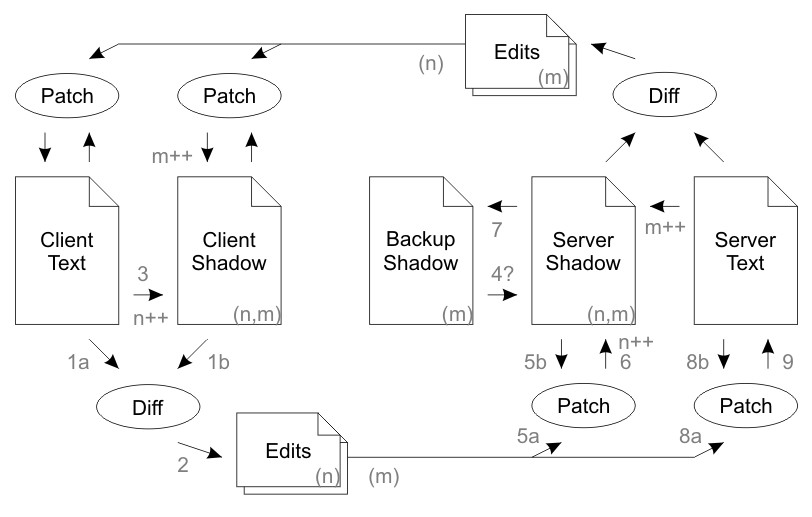
\includegraphics[scale=0.45]{diff2}
\end{figure}
\par The main difference is that in this archtitecture server has another shadow text called Backup shadow to maintain the last version of server shadow and both client and server maintain list of edits that were sent and not acknowledged, in \cite{Fraser} is this list called outbound stack. Also the versions of Client shadow and Server Shadow are labled with version numbers to be able to detect a failure in communication and acknowledge messages.
\par Basic scenario, that is presented on the picture can be described as follows:
\begin{enumerate}
\item Client text and Client Shadow are used as arguments for diff algorithm.
\item List of edits is produced and labeled with Client Shadow version \(n\).
\item Client text is copied to Client Shadow and its version is incremented.
\item This step is used only in specific situations that are described later
\item List of edits together with last known Server Shadow version number \(m\) is sent to server. This list of edits and the current Server Shadow are used as arguments for patch algorithm. 
\item Server patches edits to its shadow and increments last known client shadow version number.
\item Server takes backup of the current server shadow by copping it in the Backup Shadow. Backup shadow contains also \(m\).
\item List of edits and Server Text are used as arguments for the patch algorithm.
\item Output of patch algorithm is used to patch the Server Text.
\end{enumerate}
\par And again the process repeats simetrically, only exception is that client doesn't take a backup of his shadow. Every time one of the sites recieves an acknowledgement of its edits (\(m\) or \(n\)), it can delete these edits from outbound stack.
\par This was a description of a normal scenario without failures. To prove that this new architecture is more robust, in the following section some other scenarios will be described.
\begin{itemize}
\item \textbf{Lost data sent from client} - List of edits sent from client to server is not acknowledged. Client keeps edits in the stack and after the timeout, client sends new edits together with these old not-acknowledged edits. This repeats until server acknowledges some data.
\item \textbf{Lost data sent from server} - Server sends list of its edits together with acknowledgement of last client edits. Packet never reaches the client. Client sends new edits together with old edits (because "old" edits were never acknowledged and also never deleted from outbound stack of client). Server spots that version number \(m\) recieved from client doesn't mach version number \(m\) on server, but it maches \(m\) in backup shadow. It copies the backup shadow to server shadow (step 4 from basic scenario above), applies new edits recieved from client and coputes new diff for all edits made by server and never acknowledged by client and sends it.
\item \textbf{Duplicate packet} - When server recieves two packets from client with same number \(n\) edits from first one are applied and second one is thrown away and the communication continues as usual.
\item \textbf{Out of order packet} - The combination of scenarios mentioned above is used. One of lost data scenarios is used and then duplicate packet scenario.\cite{Fraser} 
\end{itemize}
\par The last part of this section is dedicated to diff and patch algorithms. 
\par \underline{\smash{Diff algorithm}} has two main roles in this technique. It is used to retrieve the list of edits made by user and also to save it in suitable format. Detection of user edits can be sometimes tricky and there arises the problem of semantic diff versus minimal diff. Minimal diff is in most cases not suitable for this implementation, there is a possibility that user's intension would not be preserved. For example, the change of word 'win' to 'kid' can be described as replacement of two letters 'w' and 'n' (minimal diff), but also as a replacement of whole word (semantical diff). When one side changes word 'win' to 'kid' and the other changes the word 'win' to 'won' the result should be either 'kid' or 'won', which are results of semantical diffs, the word should not be 'kod', which is result of minimal diffs. "An algorithm must be used to expand minimal diffs into semantically meaningful diffs." \cite{Fraser}
\par \underline{\smash{Patch algorithm}} takes the edits produced by the diff algorithm and patches them to the target text. This algorithm has a role of determining where to patch these edits, because the place where the desired word was at the time of edit could have changed. It has to solve a dilema whether the patch should be applied at the section with smallest Levenshtein distance \cite{Levenshtein} between two versions of the document or it should be applied at the section close to the original location. "It is probably more correct to apply a patch onto a near-match at the expected location than to a perfect match at the other end of the document."\cite{Fraser}
\par Other important property of the algorithm that need to be defined in the implementation is the length of timeout. Short cycle has higher requirements on the network, because DS is constantly sending some information over the network. On the other hand, with long cycle it is necessary to transfer bigger amounts of data and the probability of collision during patch is higher. Neil Fraser also mentions in his work that with rising number of clients scalabilty may become an issue.
\section{Commutative Replicated Data Types (CRDTs)}
\par The third technique discussed in this paper is called Commutative Replicated Data Types. Although \cite{Shapiro-long} describes CRDTs that are used in various situations, for example as implementation of registers, counters, sets, graphs, and sequences, as the main source of information for this section serves the first and most detailed work Designing a commutative replicated data type \cite{Shapiro-design} and later updates and improvements \cite{Shapiro-editing} \cite{Shapiro-consistency} This papers suggest the use of Treedoc for cooperative editing, this data structure is described later in this section. 
\par Interesting property of this technique is that CRDTs converge without any need of concurency control algorithm. This is also the reason, why this section deals mainly with the architecture of the data type and not with the technique as a whole like in the previous sections. Many papers deal with this datatype and highlight its suitability for cooperative editing. \cite{CRDT-real} evaluated CRDTs for real-time collaboration and found out that this approach is suitable for real-time collaboration, in fact the paper says that they are better in some aspects than other algorithms. This approach is used in WOOT collaboration system \cite{WOOT} and also in Logoot \cite{Logoot}, these two algorithms are briefly described at the end of this section. 
\par "A Commutative Replicated Data Type (CRDT) is a data type where all concurrent operations commute with one another." \cite{Shapiro-design} Operations commute when two sites that started in a same state apply the operations in different order and the resluting state is also the same. Achieving this property is equivalent to preserving user's intention.
\par This approach also assumes the replication of document on all sites of the collaboration and unlike the first two techniques this one doesn't use a client-server model in its implementation, instead it uses peer-to-peer architecture.
\par The smallest unit that can be inserted or deleted is called atom. This can be a character but also a larger part of the structure, for example in XML could be as atoms considered whole tags. Supported operations are instert(pos,atom) and delete(atom). 
\begin{itemize}
\item insert(pos,atom) - inserts new atom at position in document
\item delete(pos) - deletes atom at the position 
\end{itemize}
Using these two operations it is possible to produce all other needed operations. It is also easy to implement transactions using CRDTs. 
\par Every atom has its unique position identifier, it is called UID. This UID is used as parameter during execution of the operations. Properties of UIDs are:
\begin{itemize}
\item Identifier is unique and stays the same for every atom for whole life of the document.
\item There exists a total order of identifiers.
\item It is always possible to generate new identifier between any two identifiers. Generally, for any two identifiers \(A\) and \(B\), such that \(A < B\) we are able to create new identifier \(C\), such that \(A < C < B\).
\end{itemize}
Fundamental principle of this technique is that operations are executed localy and sent over the network to all other peers. There should be no need to preserve the order of the operations, this is due to commutativity property and the uniqueness of identifiers. This uniqeness also ensures that there is no need to transform operations or provide suitable context because it is clear what atom should be edited.
\cite{Shapiro-design} points out that real numbers are suitable for the role of identifiers, but for implementation it would be necessary to be able to work with infinite precision and that is imposible. The solution suggested by \cite{Shapiro-design} is the use of Treedoc. Algorithms using CRDTs differ mostly in the way of generating/maintaining these identifiesrs.
\par Treedoc is an abstract data structure that is used in document editing. It is implemented as a binary tree and every node represents an atom in the structure. The UID is the path in the tree that starts in the root. Root's UID is empty string []. Figure~\ref{fig:treedoc} shows an example of this treedoc.
\begin{figure}[H]
\caption{Treedoc}
\label{fig:treedoc}
\centering
\vspace{5mm}
\includegraphics{treedoc1} 
\end{figure}
\par Treedoc in figure encodes string 'uvwxyz' and uses characters as atoms. The UIDs for the characters are: u = [00], v = [0], w = [01], x = [], y = [1],\\z =[11]. This structure ensures the property, that it is always possible to generate new identifier between two existing UIDs. 
\par In the end, the whole document consists of pairs (UID,atom). These are ordered by UIDs. Partial order definition on identifiers can be found in \cite{Shapiro-design} and also \cite{Shapiro-editing}. 
\par Delete operation is easy to implement. Deleting is simply replacing the atom in the node with null. If the deleted atom was a leaf it can be completely removed from memory, if it was an inner node it is kept in memory and garbage collected at some point in future. However, the leaf can be completely deleted only when the delete operation is stable, which according to \cite{Shapiro-design} means that has been executed on all sites of collaboration. This paper also introduces a new procedure gc(N), which removes leaf N if it is stably deleted. This operation is executed only localy.
\par Insert opearation is harder to implement. The basic algorithm implementing this operation is not trying to keep the tree balanced, that is resolved later by other suitable solutions. Full code of the algorithm can be seen in \cite{Shapiro-design} \cite{Shapiro-editing}. 
\par Inserting new atom between to other atoms(atom\(_a\) and atom\(_b\)) is more complicated. First, the algorithm has to check if there is some atom between supplied atoms, the reason for this is that the algorithm has to insert new atom between two already present atoms that have nothing between them.
In the next step, algorithm figures out whether one of atoms is ancestor of the other, there could be 3 situations:
\begin{itemize}
\item atom\(_a\) is ancestor of atom\(_b\): In this situation, atom\(_b\) has no left child so this new atom will be new left child of atom\(_b\). New UID will be \(uid(b) \cdot 0\)
\item atom\(_b\) is ancestor of atom\(_a\): In this situation, atom\(_a\) has no right child so this new atom will be new right child of atom\(_a\). New UID will be \(uid(a) \cdot 1\)
\item atoms are not in ancestry relation:  In this situation, atom\(_a\) has no right child so this new atom will be new right child of atom\(_a\). New UID will be \(uid(a) \cdot 1\)
\end{itemize}
\par Ancestry relation is defined as expected. The node \(a\) is ancestor of node \(b\) if on the path from \(b\) to root node there is \(a\). This also means that \( uid(b) = uid(a) \cdot (0,1)^k \) where \(k\) is the diference between depths of these two nodes.
\par The problem with concurrent inserts is resolved with extension of the nodes with disambiguators. These disambiguators are pairs of \(idX = (siteID, counter)\) where \(siteID\) represents the site that iniated the creation of this disambiguator and \(counter\) variable represetns counter that is maintained by each site. There is also a total order of disambiguators defined: \( (s_1,c_1) < (s_2,c_2) \quad iff \quad c_1<c_2 \vee (c_1=c_2 \wedge s_1 < s_2) \) This ensures that every disambiguator is unique and that the order of disambiguators is same on every site. 
\begin{figure}[H]
\caption{Treedoc}
\label{fig:treedoc2}
\centering
\vspace{5mm}
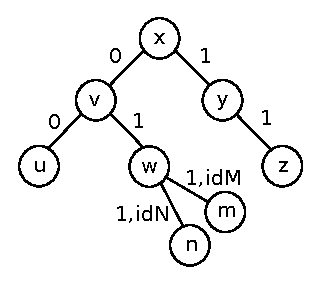
\includegraphics{treedoc2} 
\end{figure}
\par Figure~\ref{fig:treedoc2} shows the use of disambiguators. As this concurrency can occur at every node, \cite{Shapiro-design} suggests the use of disambiguators on every node when it is created and garbage collecting these disambiguators periodically. An insert opeation is stable at some site, when this site recieved all operations that happened after this operation has been executed localy from all sites. At this point it is clear that there will be no other concurrent inserts. 
\par The last opeartions designed for this abstract data structure are \textit{explode(string)} and \textit{flatten(path)}. Operation \textit{explode(string)} accepts a string of atoms and returns a tree, that is consruted from supplied string and operation \textit{flatten(path)} accepts a path from sub-tree and returns a string of atoms. Flatten operation skips the null nodes on the path. These nodes where produced by deleting inner nodes. Sequntial application (\textit{explode(flatten(treedoc)}) of these two operations on an unbalanced treedoc with null nodes results in new treedoc that has the same content, but it is balanced and without null nodes in the structure. These operations don't commute with edit operations on the tree. The \textit{explode} operation is not really necessary, it can be substituted with aplying a path to a string. So there is no need to search for solution for its commutativity. The commutativity of \textit{flatten} operation is ensured by voting. This operation can not be executed when there is another \textit{insert} or \textit{delete} in progress. Therefor, all the sites vote whether the flatten operation can be executed. If one of the sites spots an edit operations it votes "No" otherwise it votes "Yes". \textit{Flatten} is executed only if all sites vote "Yes".
\par Interesting thing about CRDTs is that with this approach it is easy to implement transactions. As the operations commute all that is needed are labels of the begining and the end of the transaction and a buffer. When a peer executes local transaction all operations recieved from network are buffered and vice versa. With transaction support it is easy to implement block operations such as copy and paste or search and replace. Because we can guarantee that during the transaction the state of the document won't change.
\par Last part of this section deals with Logoot and WOOT algorithms, which are alternatives to the original algorithm. They both use the idea of CRDTs, so every atom has its unique identifier an that is the reason why there is no conflict in the execution of the operations and the operations commute. They also use only 2 operations that were descirbed earlier. The only difference is in the way of generating the identifiers. 
\par Logoot tries to avoid the use of thombstones, which are deleted atoms that had to remain in the structure, but they are not visible. (e.g. null nodes in Treedoc). It has a bit more complicated structure for the UIDs and it uses whole lines as atoms. Every site has its site identifier \(s\) and a "clock" \(h_s\) that is incremented every time a line is created. Every line has its position \(pid\) in the document. Position is a list of identifiers and identifier is a couple of \(<p,s>\) where \(p\) is an integer and \(s\) is the unique site identifier. Whole document consists of pairs \((pid,text)\). Also the first and the last line are uniquely identified by having \(l_B\) (beginning) and \(l_E\) (end) in the text variable. Example line generated by site \(s\) can look like this: \( ((<i,s>,h_s),text) \). New UIDs are generated by addning more identifiers (\(<i,s>\)) in the first part of the position tuple and by updating \(h_s\). The order of the identifiers can be described as lexicographic. Authors of Logoot point out that the use of thombstones genereates big overhead, so they tried to avoid it by using new format of identifiers. More information can be found in \cite{Logoot}.
\par WOOT is one of the first algorithms that used CRDTs. The time complexity is not as good as Logoot's time complexity, this is caused mainly by thw use of thombstones. WOOT identifies characters as atoms and every character has a unique identifier, this atoms are called W-characters. This W-character is a tuple \( <id,\alpha,v,id_{cp},id_{cn}> \) where \(id\) is the identifier of the character, that is a cuple constructed of unique identification number of the site and a logical clock. \(\alpha\) is the actual value of the character. \(v\) is bolean value that represents visibility and \( id_{cp}, id_{cn} \) are identifiers of the previous and next character. These identifiers are the reason why there have to be the tombstones, they are necessary to indetify the exact position of the character on each site. Partial order between the atoms is defined and uniqness of the UIDs is ensured by a unique indetifier of the site and with the logical clock. The supported operations are also insert and delete. 
\chapter{Comparison of Techniques}
The following chapter will present a comparison of these thechniques using the criteria described in the following section. This chapter belongs to the teorecital part of the thesis, so the comparison is more general. It points out the general advantages and disadvantages of these techniques. 
\section{Comparison Criteria} \label{comparison}
This section describes the comparison criteria for the presented techniques and presents the reasons for choosing these particular criteria. These criteria together with other requirements are used in the section \ref{requirements} for desciribing Komodo requirements for real-time collaboration and in section \ref{best} for choosing the best technique.
\par Comparison criteria include:
\begin{itemize}
\item client-server vs. peer to peer model
\item requirements on local machine vs. remote machine
\item amount of data transfer
\item network requirements
\item time complexity
\item conflict resolution ability
\item latency tolerance
\item supported content formats
\end{itemize}
\par It is important to determine whether the technique can be used only with client - server model or with peer to peer model or with both of them. With this requirement also related the scalability of the technique, how many participant could be in the collaboration. This is important for the use in practice, because this can be one of the most fundamental requirements of the system. When evaluating this creteria, we assume that the number of collaboration sites is greater than two.
\par One of the comparison criteria are performance requirements. These requirements should be reviewed as requirements on local machine vs. requirements on remote machine. Some techniques might have harder requiremts on the user side and other on server side.  Evaluation of these requirements is also dependent of the architecture.
\par The amount of data transfer is also important. The more data is necessary to transfer the harder it is to implement this technique in enviroments with collaboration sites in distinct parts of the world. Best practice is to transfer as few data as possible. This criterion should be reviewed in costrast with other techniques.
\par Network requirements should be taken into account, because it is necessary to know if one of the techniques requires particular protocol or some other network functionality. Some of the technniques may not be suitable for bigger networks like Internet, they may be suitable only for local area networks.
\par Time complexity is very closely related to the requirements on the machines. This creterion focuses on the time complexity of the algorithms that ensure consistency maintanance. Some of the techniques might do the majority of the work in the algorithm, other may have done some preparation and the following algorithm is not so complex.
\par Conflict resolution ability is also assessed. The main goal is to have as few conflicts as possible, but when some conflict occurs, it is necessary to resolve it as fast as possible and with the correct result. All of the techniques are able to resolve conflicts, but the important part is the correctnes of the result. 
\par The best technique should be also able to tolarate the latency of the network. The ability to recover from lost packet situation or recover from situation when the packets come out of order is important. 
\par The last criterion in ability to process various content formats. This part should point out the which formats are supported and which are not supported by particular technique.
\section{Comparison}
\par This section evaluates the techniques according to presented criteria. The main part is devieded by techniques and by each technique all criteria are evaluated. In the last part of the comparison a table will be presented to summarize the findings of this section.
\\
\par \textbf{\underline{\smash{Operational transformation}}}

\vspace{3mm}

\textbf{Client-server vs. peer to peer model} - All articles about Operational Transformation used in this thesis suggest the client - server model for this technique. The main reason why this technique can not be implemented with peer to peer model is the fact, that client has to send operations that come from a state in server's history. This would imply that every peer would have to preserve history of every other peer to be able to send such operations. This problem already occured in the design of Operational Transformation, and was resolved by moving the resposibility to track the history from server to clients.

\vspace{3mm}

\textbf{Requirements local vs. remote} - In this technique are requirements on local machine slightly higher than on remote server. As mentioned above, client has to track server's history and send only particular type of opeations. Server solves only the basic diamond problem and sends out operations that it receives.

\vspace{3mm}

\textbf{Amount of data transfer} - Operational Transformation sends only operations over the network. Only in network failures it is necessary to transfer the whole document. The amount of data transfer necessary for this technique is low.

\vspace{3mm}

\textbf{Network requirements} - This technique assumes the use of connection over TCP protocol\cite{Jupiter}\cite{simplified}, in order to ensure the delivery. Although the mechanism should be able to detect lost packets, because server has to acknowledge operations.

\vspace{3mm}

\textbf{Time complexity} - Time complexity for consistency maintanance is linear.\cite{sequence}\cite{orthogonal} For other more specific and more difficult functions, like undo the complexity can be non-linear.

\vspace{3mm}

\textbf{Conflict resolution ability} - The transformation function is the main part that ensures good conflict resolution. The role of this function is to transform the operations against each other in order to preserve user's intension, convergence and casuality.

\vspace{3mm}

\textbf{Latency tolarenace} - As it was mentioned above, server has to acknowledge user operations. This means that the chance that user operations will get lost is very small. This also implies that server preserves a version of the document on which all operations were apllied, in case of incosistency the whole document can be transferted to user.

\vspace{3mm}

\textbf{Supported content formats} - Operational transformation is able to process plain text, but also variety of other formats like XML and other tree structured data types. This technique is used also in graphics editing systems\cite{graphics} like CoFlash and also for collaborative slides creation and presentation CoPowerPoint.

\vspace{3mm}

\par \textbf{\underline{\smash{Differential Synchronization}}}

\vspace{3mm}

\textbf{Client-server vs. peer to peer model} - This technique is also not suitable for peer to peer model of architecture. It would be really computationaly complex for each client to maintan \((n-1)\) peer shadows and to compute \((n-1)\) diffs, also the patching would be really hard. With rising number of peers the real-time collaboration would be impossible to implement.

\vspace{3mm}

\textbf{Requirements local vs. remote} - Differential sychronization has harder requiremts on server than on client. Niel Fraser \cite{Fraser} points out that the algorithm is symetrical, which means that (nearly) identical code is running on all machines, but the final version of the algorithm presented in his paper is more difficult for server. It has to maintain another shadow for the case of dataloss and server is also responsible for broadcasting the operations to every client and for patching all operations on its document version.

\vspace{3mm}

\textbf{Amount of data transfer} - Data transfer might be the highest among these techniques because the changes made in document described in a diff file are provided with context, in order to find ther right place for paching.

\vspace{3mm}

\textbf{Network requirements} - No special properties of network are necessary for this technique. Differential synchronization has a good mechanism that is able to recover from loss of packet so it can be implemented also over UDP protocol.

\vspace{3mm}

\textbf{Time complexity} - Time complexity depends on diff and pach algorithms and can differ with the content format and with the choice of these algorithms as there can be more algorithms for particular content format. For example, one of diff algorithms for XML file is XyDiff\cite{Xdiff} and this algorithm achives \(O(nlogn)\) complexity in execeution time.

\vspace{3mm}

\textbf{Conflict resolution ability} - This property depends on patch algorithm. One of roles of this algorithm is to identify the conflict and be able to resolve it with correct result. The choice of the algorithm is free so it can not be evaluated in general.

\vspace{3mm}

\textbf{Latency tolarenace} - There is a good guranteed delivery method used in this technique that is described in the previous chapter. Almost every situation can be resolved without having to send the whole document over the network.

\vspace{3mm}

\textbf{Supported content formats} - Differential synchronization can be used with every format as long as there are diff and patch algorithms present.

\vspace{3mm} 

\par \textbf{\underline{\smash{Commutative replicated data types}}}

\vspace{3mm} 

\textbf{Client-server vs. peer to peer model} - Peer to peer archtitecture is presented in most cases for this approach. Sites of collaboration only send the operations that have been done locally so there is an option to broadcast the operations to every peer and also to send operations to one server that will take care of broadcasting operations to other clients.

\vspace{3mm} 

\textbf{Requirements local vs. remote} - Requirements are equal on each site of the collaboration. Every site has to maintain correct order of identifiers and send\textbackslash receive operations. This also depends on the architecture. If a client-server model is choosen, the requirements on server would be heigher because server would have to broadcast the messages.

\vspace{3mm} 

\textbf{Amount of data transfer} - Amount of data transfer in this approach is comparable to the amount neede in Operational Transformation. Atoms of the document are uniquely identified, so there is no need to provide context, only the operations and the identifier of the atom are sent over the network.

\vspace{3mm} 

\textbf{Network requirements} - Network requirements of CRDTs are not special. One of the reasons could be, that this technique concerns mainly with the identification of the atoms and doesn't concern with the newtwork problems, such as packetloss or packets that are out of order.

\vspace{3mm} 

\textbf{Time complexity} - Time complexity is depenedent on the choosen type of identifiers and with the algorithm that generates new identifiers. The technique itself only sends operations over the network, keypoint is the ability of the algorithm to generete new identifier or to find the correct place for insertion of new atom. It can not be evaluted in general as it was by Differential Synchronization. For example, according to \cite{CRDT-real} WOOT has a worst case time compexity of insert operation equal to \(O(n^3)\) and time complexity of delete is equal to \(O(n)\) where \(n\) is the number of atoms. Time complexity information for other algorithms can be also found in \cite{CRDT-real}.

\vspace{3mm} 

\textbf{Conflict resolution ability} - Every atom is uniquely identified so there should be no conflict. Where there are two concurent operations that try to delete same atom, the second delete operation will find a tombstone and assume that is has been already deleted. Concurency of two insert operations at the same place is resolved individualy by each algorithm that generates identifiers.

\vspace{3mm} 

\textbf{Latency tolarenace} - As it is mentioned above, this techniques deals mainly with identification of the atoms, so the mechanism for latency tolerance is very weak. Every site basicly logs its operations (both local and remote). New site or crashed site will recieve whole document and a site that was disconnected for a while recieves all missing operations.

\vspace{3mm} 

\textbf{Supported content formats} - This technique can also support any format of content. The fundamental element is the devision of the content to atoms and their identification. 

\vspace{13mm} 

\noindent
\begin{tabular}{| p{1.7cm} | p{2.2cm} | p{2.2cm} | p{2.2cm} | p{2.2cm} |}
\hline
 & C-S vs. p2p & local vs. remote* & data \newline transfer & network req.  \\
\hline
OT & C-S & local & low & use of TCP assumed \\
\hline
DS & C-S & remote & higher & no special \\
\hline
CRDTs & both & equal & low & no special \\
\hline
\end{tabular}
\newline
\vspace*{1 cm}
\newline
\begin{tabular}{| p{1.7cm} | p{2.2cm} | p{2.2cm} | p{2.2cm} | p{2.2cm} |}
\hline
 & time** \newline complexity & conflict resolution*** & latency tolerance  mechanism & content formats \\
\hline
OT &  \(O(n)\) & X & average  & any \\
\hline
DS & \(O(nlogn)\) & X & strong  & any \\
\hline
CRDTs & \(O(n^3), O(n)\) & X & weak  & any \\
\hline
\end{tabular}
\vspace{10mm}
\newline
* Table discribes on which site are the requirements higher. \newline
** By all techniques time complexity is dependent on implementation, time complexities are only informative. \newline
*** Conflict resolution ability can not be compared in this table. In each case this ability depends on choosing particular function/algorithm.
\chapter{Red Hat JBoss Data Virtualization}
\par This chapter covers the practical part of the thesis, it describes briefly Red Hat JBoos Data Virtualization platform, an Eclipse-based design tooling called Teiid Designer and its new upcomming version Komodo. In the next section, it presents requiremets of Komodo for real-time collaboration and the following part deals with choosing the best technique for Komodo from three presented techniques in the theoretical part. The last part deals with Java implementation of this technique that can be used in acctual implementation of real-time collaboration in Komodo.
\section{Overview}
\par Red Hat JBoss Data Virtualization platform is a product based on community project called Teiid.  This software is able to federate and itegrate data sources of all kinds, like SQL datasources, non-SQL databases, Flat files, XML files, Excell files, webservices and more. It makes development of new applications easier, because the software developer doesn't have to query every datasource that his new application needs and federate the data in his application, Datava Virtualization platform will do this for the developer.
\par This platform is able to create one virtual database called VDB that will federate all underlying datasources and make it look like there is only one datasource. It runs on top of aplication server called Red Hat JBoos Enterprise Aplication Platform.
\par Users of this product are able to create VDBs 2 ways. One is to manually create an XML file with certain structure, this VDB is called dynamic VDB. In this VDB the user describes what datasource defined on server they want to use, there is also a security mechanism that is able to limit the access only for certain users and user can specify all needed information for federation of the datasources.
\begin{figure}[H]
\caption{Red Hat JBoss Data Virtualization}
\label{fig:dv}
\centering
\vspace{5mm}
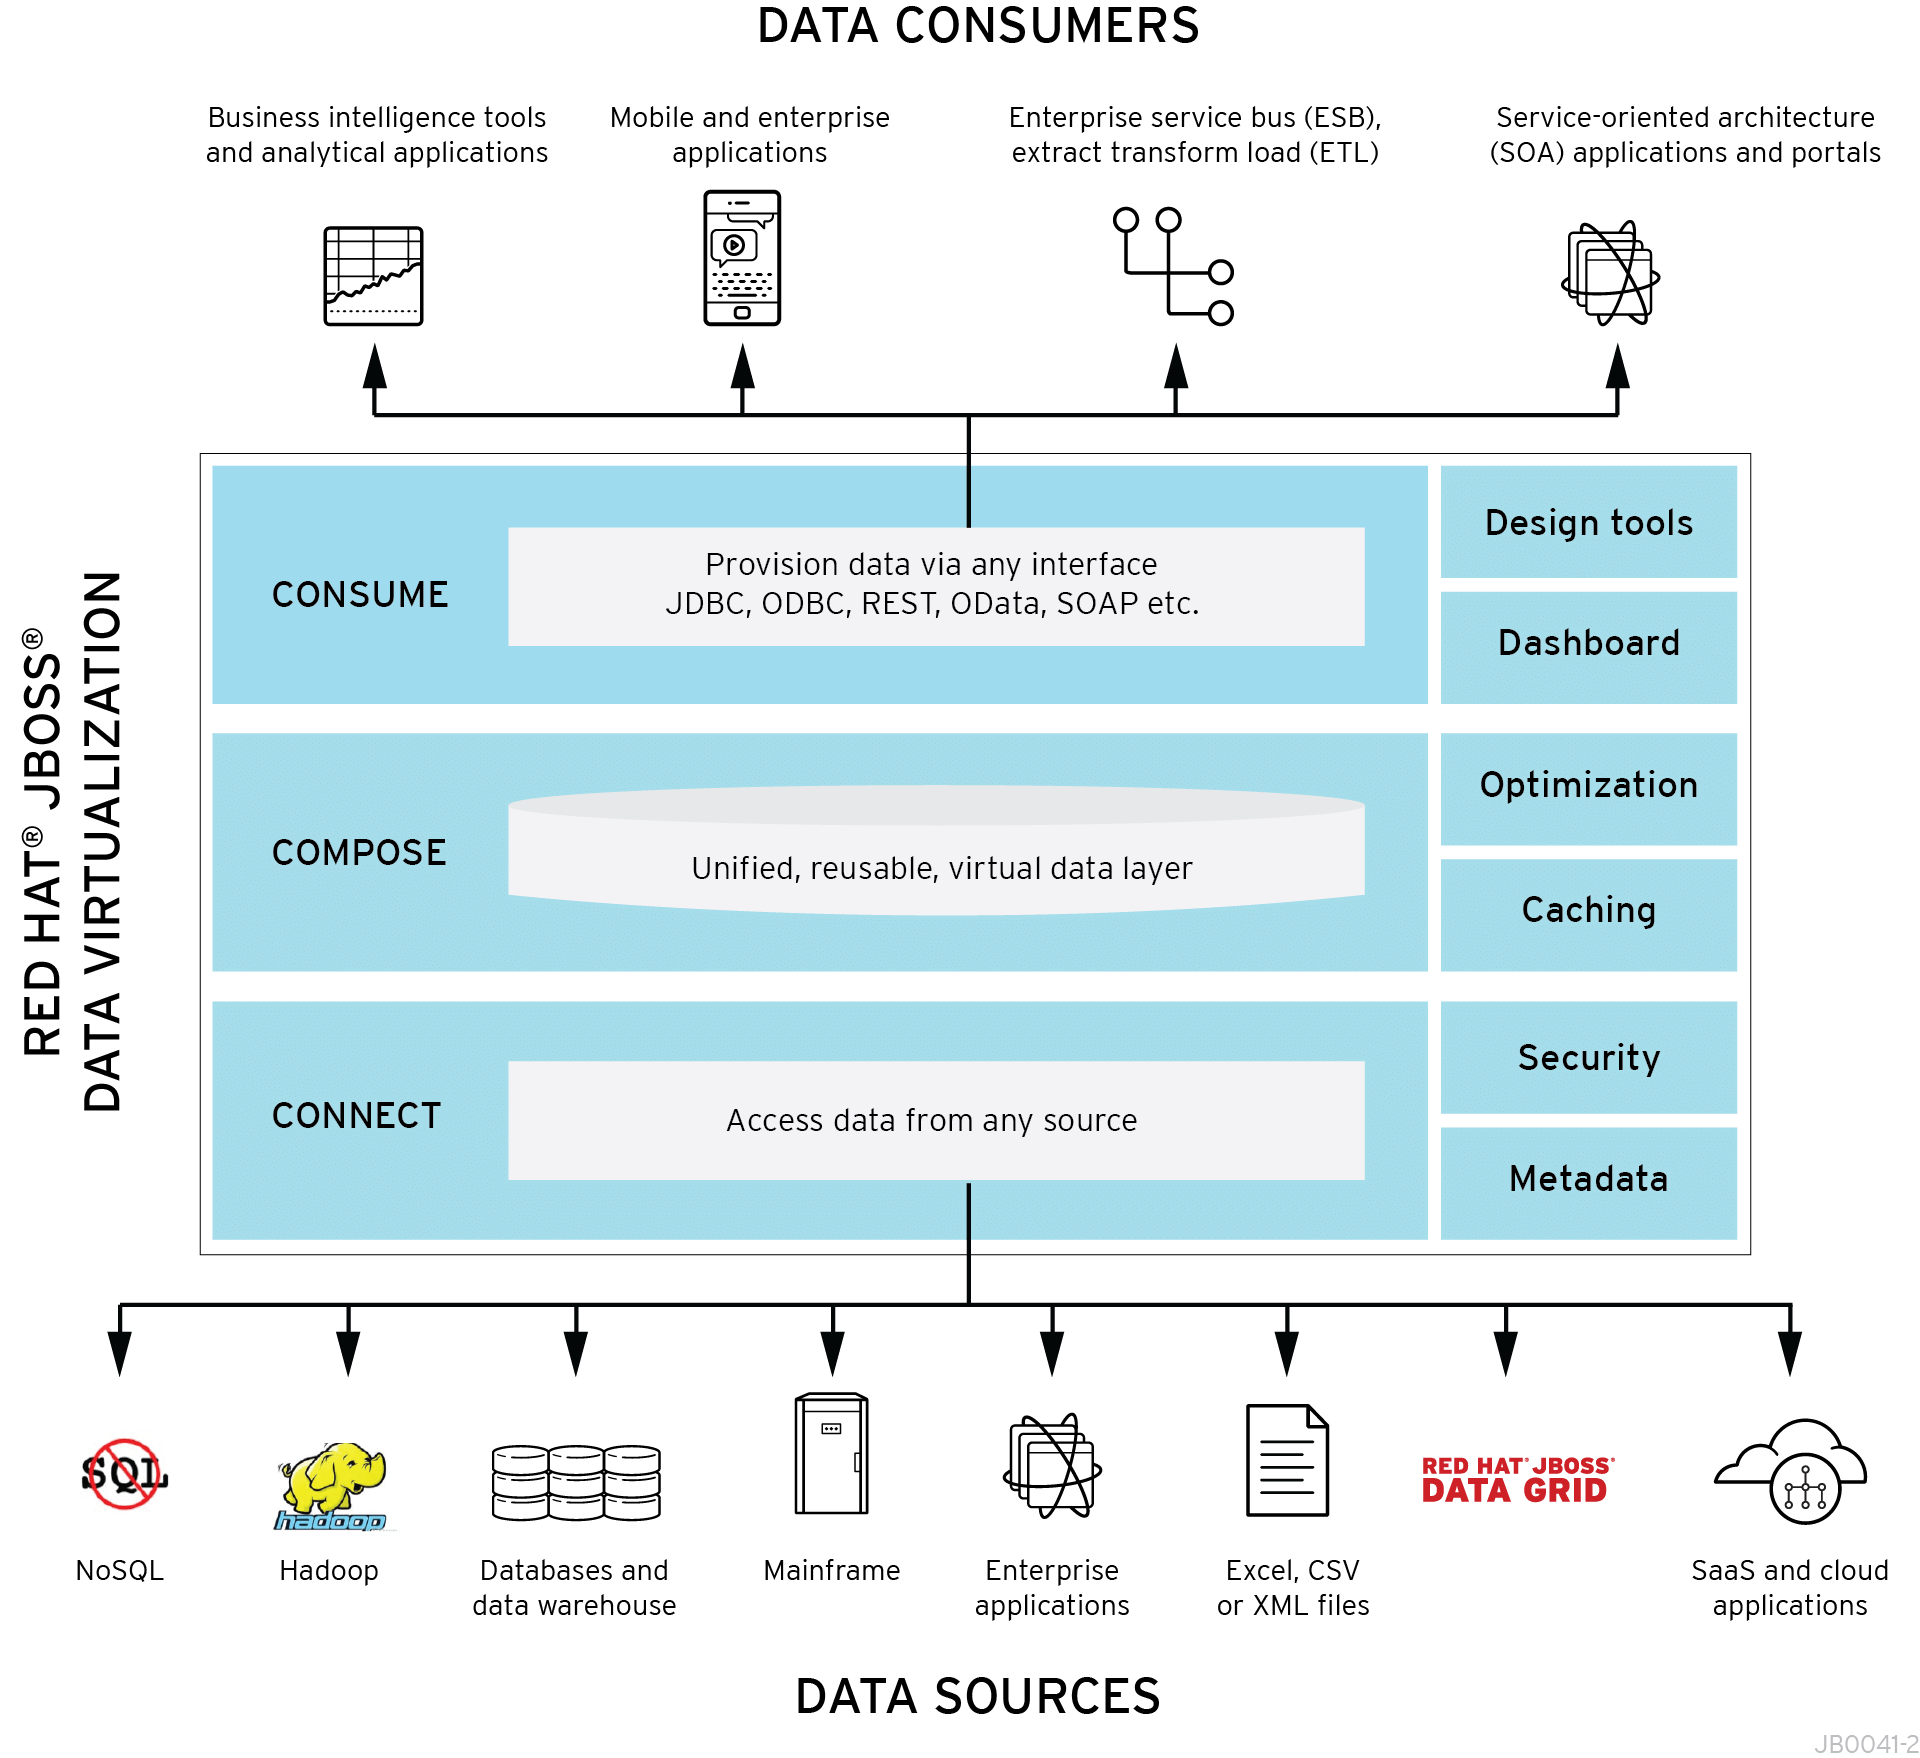
\includegraphics[scale=0.15]{dv} 
\end{figure} 
\par Another alternative is to create a project in Teiid Designer. Teiid Designer is an eclipse-based designing tool for Data Virtualization. Using this tool it is much easier to create connections to remote and local datasource and also to federate them. User imports metadata from various datasources. These metadata about a datasource are represented in Teiid Designer by a Source model. User can specify which tables, columns or another type of structure they want to include in their project. There are also View models present, in which user can specify the federation schema and alter the structure of the tables provided by Source model. We can say that Source model represents the physical data storage and View model represents a business view of the data. At the end the models are included in a static VDB file. Static VDBs are also files with XML structure but they are more complicated and not easy to create without tooling. 
\par These VDBs are then deployed to Teiid server and external users/applications can query this new database. This VDB acts as one SQL database and doesn't expose the internal structure. User can choose also to produce a web service instead of a VDB. 
\par Another benefit of Red Hat JBoss Data Virtualization is also the fact, that it enables quering datasources that are not easy to query without Data Vritualization, these datasources are for example Flat files, XML files and Excel spreadsheets. Teiid has a set of translators that are able to "translate" the content from various formats to teiid server logic.
\section{Komodo}
\par This section should provide some basic information about Komodo and the differences and improvements that will be included in Komodo. All information about Komodo that are presented in this section are from members of Komodo developing team or from Komodo Release Development plan \cite{Komodo}. 
\par Komodo should be a new version of Teiid Designer, which has has many new features and tries to get the designing tool closer to Teiid server. The main impulses for creating a new tooling for Data Virtualization were changes in Teiid 8.x and the use of dynamic VDBs in Openshift platform.  
\par The fundamental difference in architecture of this tool is the division in two parts. The KEngine and User Interface (UI). KEngine will be the main part that will handle all necessary functionality an will form the core of the application. This engine should adapt the common Teiid DDL dialect for relational data definition. KEngie will have Command Line Interface (CLI) through wich all activies will be possible to perform. User will be able to choose between CLI and UI.
\par At the time of writing this thesis the CLI is beiing finalized. User will be able to create models and VDBs using few simple and understandable commands like CREATE, RENAME, DELETE, SET and others.
\par User Interface will provide a clickable interface for users, to this day it was not decided if the UI will be web-based or Ecplise-based. New UI should not include Eclipse modeling framework used in Teiid Designer.
\par Another change in Komodo is the use of ModeShape as a place for storing information about models and VDBs. Komodo won't use Ecplise workspace anymore. It should use KSpace , which will be a new workspace that is based on JCR e.g. ModeShape. 
\par "ModeShape is a distributed, hierarchical, transactional, and consistent data store with support for queries, full-text search, events, versioning, references, and flexible and dynamic schemas."\cite{ModeShape} It implements the JSR-283\footnote{\url{https://jcp.org/en/jsr/detail?id=283}} standard Java API from content repositories also known as JCR. This kind of repository is a suitable solution for Komodo because it is good at storing hierarchical data, file storage also versioning and many other aspects. 
\par Data in ModeShape are stored in a form of nodes connected to each other.  ModeShape has some basic node types deifned, but in most cases it is necessary to define custom nodes for the desired application. This definition of node types is called Compact Node Definition. Komodo nodes in repository will be Teiid Dynamic Artifacts. These artifacts are for example models, tables, colums, DDL statments and so on. Komodo has already prepared majority of these defiinitons\footnote{\url{https://raw.githubusercontent.com/Teiid-Designer/komodo/master/plugins/org.komodo.modeshape.teiid.sql.sequencer/cnd-examples/StandardDdl.cnd}}\footnote{\url{https://raw.githubusercontent.com/Teiid-Designer/komodo/master/plugins/org.komodo.modeshape.teiid.sql.sequencer/demigen/org/komodo/modeshape/teiid/cnd/TeiidSql.cnd}}. There is also a suggestion to use multiple local KSpaces and also remote KSpaces for the collaboration purposes. 
\par One of major changes in approach of the modeling in this new tool, is that the creation of new VDB should be "VDB-centrinc" instead of "Project-centric". In other words the creation of VDB in Teiid Designer begins with creating a Model Project, as a next step user creates models and then they include these models in a VDB which is deployed to the server. Komodo won't use Projects, user will create an artifact an then it could be saved in a local library for later use. The workspace concept contains VBDs and/or models.\\ \\
The major conceptual changes can be summarized in six points:
\begin{enumerate}
\item \textbf{Simplify terminology }- terminology of Teiid Designer is sightly different from the terminology used by Teiid. Komodo should eliminate these differences.
\item \textbf{Replace the notion of "Source models" with "Data sources" }- This point is in strong relation with the first one. It is more understandable to name the base models as Datasources, as this terminlogy is also used by Teiid server.
\item \textbf{Expose Create Views or Virtual Procedures as primary feature} - There is an effort to remove the diversity of models, Teiid Designer has a lot of model types such as Source, View, Relational, Web Service, XML and other. The number of models should be cut down and user will use simplier DDL constructions.
\item \textbf{Exapad notion of a VDB in the workspace} - Komodo will implement Teiid's Dynamic VDB functionality
\item \textbf{Ability to connect to multiple KSpaces} - Komodo will add an ability to have multiple local or remote workspaces as it was already mentioned above.
\item \textbf{New global workspace location concept} - Stadard eclipse workspace has many drawbacks, for example when users switches workspace the connection profiles have to be exported from old workspace and reimported into the new one. Global workspace should store these common data outside of regular workspace.
\end{enumerate}
\section{Komodo Requirements for Real-time Collaboration} \label{requirements}
\par This section describes the requirements on real-time collaboration that are set by Komodo software. All information presented in this section also come from \cite{Komodo} or from conversations with development team.

\vspace{3mm} 

\textbf{Architecture model} - Komodo is able to use Client - Server model in its implementation of the real-time collaboration. This approach seems to be more reliable and suitable for real-time collaboration. This is in relation with the requirement for number of collaboration sites.

\vspace{3mm} 

\textbf{Remote vs. local requirements} - There is no specification on wich side the requirements should be greater. Server will have to broadcast the changes and maintain a server version of the document, which means it will have to recieve changes from number of clients, on the other hand client deals with the actual modeling of the artifact and also with sending and recieving messages.

\vspace{3mm} 

\textbf{Amount of data transfer} - Obviously, the amount of data transfer should be as small as possible. In order to make the technique as fast as possible. The VDB files are as small as they can be, because they don't hold any data and store only DDLs for transformation of data into desired format.

\vspace{3mm} 

\textbf{Network requirements} - Komodo doesn't have any special network requiremts. Only requirement is that real-time collaboration should be implemented over Internet.

\vspace{3mm} 

\textbf{Latency tolerance} - As the real-time collaboration should be performed over the internet the latency tolerance should be as good as possible.

\vspace{3mm} 

\textbf{Data type} - Although Komodo will use ModeShape as a datastorage, real-time collaboration should deal with dynamic VDBs. These VBDs are in form of XML files as it was mentioned before. The structure of an example VDB.xml file can be seen in Komodo Release Development plan\cite{Komodo}. It mostly consists of few XML tags and DDL statments. This content format requirement is very important and has the main impact on the choice of the technique.

\vspace{3mm} 

\textbf{Number of participants} - The number of users collaborating on one model/vdb/artifact can be greater than two. The client-server model should be more suitable for the rising number of users. The chosen technique should be well scalable.

\vspace{3mm} 

\par Aspects of Time complexity and Conflict resolution ability are not mentioned because it is obvious that these two properties should be as good as possible.
\section{Best Technique for Komodo} \label{best}
\par This section deals with choosing from three presented techniques the best one for Komodo according to requirements set in the previous section. At the end of the section is short reasoning why we chose a CRDTs as the best technique for Komodo. 

\vspace{3mm} 

\textbf{Architecture model} - All three techniques are able to work with Client - Server model. This requirement doesn't rule out any of the presented techniques.

\vspace{3mm} 

\textbf{Remote vs. local requirements} - Komodo doesn't have limitations in this area. It is not necessary to rule out any of the techniques.

\vspace{3mm} 

\textbf{Amount of data transfer} - Operational transformation and CRDTs have the lowest data transfer. Differential synchronization seems to be less suitable for Komodo regarding this requirement.	

\vspace{3mm} 

\textbf{Network requirements} - Komodo has no special requirements for network. This aspect doesn't rule out any technique.

\vspace{3mm} 

\textbf{Latency tolerance} - Best latency tolerance mechanism is presented by Differential Synchronization, other two techniques do not significantly deal with latency tolerance in the presented papers, although it should be easy to add this mechanisms.

\vspace{3mm} 

\textbf{Data type} - All of the techniques are able to process any data format, in case of Dyfferential synchronization there should be diff and patch algorithms present for the desired data format. Operatational Transformation was implemented for Google Wave and this application worked with waves as XML files. There are also diff and patch algorithms present for XML files, one of the examples (XyDiff) is referenced in the section \ref{comparison}. CRDTs are able to process XML and might be a best solution for Komodo considering this aspect, because we can choose what part of data can be an atom for this technique. Not only whole XML tags can be considered as atoms, but also some main and stable parts of DDL such as CREATE, VIRTUAL PROCEDURE, SELECT, FROM, WHERE etc.

\vspace{3mm} 

\textbf{Number of participants} - This requirement seems to be the breakpoint in deciding what technique is the best for Komodo. As Niel Fraser \cite{Fraser} points out, there can be a scalability problem with rising number of participants by Differential Synchronization.

\vspace{3mm} 

We choose as a best technique for implementation in Komodo the technique of Commutative Replicated Data Types (CRDTs). Problem with scalability and higher data transfer in comparison with other two tehcniques rule out the Differential Sychronization as the best technique for Komodo. Operational transformation seems to be a good theoretical technique for real time collaboration, but implementing this technique on a reliable level is hard and considering real-time collaboration in Komodo as minor feature not the main feature of the software, the technique for real time collaboration should not be hard to implement. Google wave implementation of Operational Transformation, which is known today as Apache wave, is an open-source project and eventhough it could be used in Komodo, this implementation deals with XML files, it would not be easy to modify for Komodo. Positives of CRDTs are: the possibility to define larger parts of the document as atoms, low data transfer and compatibility with nearly any content type. 

\section{Java Implementation}
\chapter{Conclusion}
\bibliographystyle{acm} 
\bibliography{bib-db} 
\end{document}
